\documentclass{beamer}
\usepackage[utf8]{inputenc}

\usepackage{bookman}
\usefonttheme{structuresmallcapsserif}

\usetheme{Madrid}
%\usecolortheme{beaver}
\title{A More Consistent Understanding of Consistency}
%Information to be included in the title page:
\author[Subhajit, Ricardo, Rordigo] % (optional, for multiple authors)
{Subhajit Sidhanta\inst{1} \and Ricardo Dias\inst{2} \and Rordigo Rordigues\inst{3}}

\institute[] % (optional)
{
	\inst{1}%
Indian Institue of Technology Bhilai (IIT Bhilai)
	\and
	\inst{2}%
	NOVA LINCS, Universidade NOVA de Lisboa \& SUSE Linux GmbH
	\and
	\inst{3}
	INESC-ID / Instituto Superior T\'{e}cnico, ULisboa
}

\date[SRDS 2019] % (optional)
{SRDS, October 2019}

\logo{\includegraphics[height=1.5cm]{HD Logo of IIT Bhilai.png}}
 
 
\begin{document}
 
\frame{\titlepage}
 
\begin{frame}
\frametitle{Syntax and Notations}
 A Consistency Model : a contract (order among observed results) between the storage and the client (processor).\\

Conventions we will use:
	\begin{itemize}
		\item $\mathit{st}$: a session trace
	\item $\mathcal{S}_t$: global session trace denotes the set of all
	session traces in a given execution of the system.
	 \item $w(x,v)$: an invocation of a write operation that writes a value $v$ to an object $x$.
	\item $r(x){v'}$: a read operation on object $x$ that outputs a value $v'$
	\end{itemize}
\end{frame}

\begin{frame}
\frametitle{Consistency and the CAP Theorem}
 
\begin{columns}
	
	\column{0.5\textwidth}
	\includegraphics[height=3cm]{acid.png}
	
	\column{0.5\textwidth}
	\includegraphics[height=3cm]{CAP.png}
\end{columns}
	\begin{columns}
	\column{0.5\textwidth}
	\includegraphics[height=4cm]{Linear.png}
	\column{0.5\textwidth}
	There exists a host of different Consistency Levels between Linearizability and Eventual. One must choose an appropriate consistency model.
	
\end{columns}
\end{frame}

\begin{frame}
\frametitle{Consistency Models}

\begin{columns}
	
	\column{0.5\textwidth}
	\includegraphics[height=4cm]{rywmodel.png}
	
	\column{0.5\textwidth}
	\includegraphics[height=4cm]{causalmodel.png}
\end{columns}
Choosing appropriate consistency model requires understanding the operational  semantics of model. This makes a formal model necessary rather than textual definition.

\end{frame}

\begin{frame}
\frametitle{Implications of Different Consistency Models}
\begin{columns}
	
	
	\includegraphics[height=5cm]{implications.png}
\end{columns}
There is an ever increasing number of storage systems which implement a wide range of consistency models. 

\end{frame}

\begin{frame}
\frametitle{Motivation for formalization of consistency models}
\begin{itemize}
	 \item Large number of different models
 \item Defined using different formalisms
 \item Community-specific terms and definitions
 \item How do they compare?
 \item “The causal+ consistency (…) falls between sequential and causal consistency” [COPS]
“FJC implies a number of (…) session guarantees” [Depot]
\end{itemize}

\end{frame}

\begin{frame}
\frametitle{Unifying Specification of Consistency Models}
\begin{itemize}
	\item Goal: find a unified way to specify consistency ad isolation levels that is:
	\item Simple and intuitive
	\item Unifies consistency model definitions using a common syntax
	\item How do they compare?
	\item Directly applicable to automated verification  systems
	\item Enables straightforward comparisons of levels
	\item Allows for efficient verification of implementations
\end{itemize}

\end{frame}
 
 \begin{frame}
 \frametitle{Related Work}
 \begin{itemize}
 	\item Chockler DISC 2000: descriptive (informal) specifications
 	\item Adya’s Generalized isolation levels: \\
 		Similar goal applied to isolation levels but applicable only to version based systems\\
 		Isolation levels defined by precluded cycles in dependency DAG's
 	\item Cerone: Complex Algebraic rules based on dependency relations assuming system specific arbitration mechanisms
 	\item Attiya PODC 16: Consistency semantics tied to replicated systems
 	\item Lacking support of automated tools
 	
 \end{itemize}
 We wish to make definitions implementation agnostic and simple
\end{frame}
 
 \begin{frame}
 \frametitle{Terminology}
 
 We use a shorthand notation $W^{x}_{st}$ to denote a variable that refers to a write operation to object $x$ that is part of session trace $st$. \\
 In turn, the notation $R^{x}_{st}$ denotes a read operation to object $x$ in session trace $st$.\\
 
 For instance the LTL formula
 
 $$ \quad \square \left( R_\mathit{st}^x \rightarrow \lozenge W_\mathit{st}^{x'} \right) $$
 
 \noindent is satisfied by any session trace $st$ where, if a read operation on object $x$ is issued, then it must be eventually followed by a write operation on object $x'$.
 	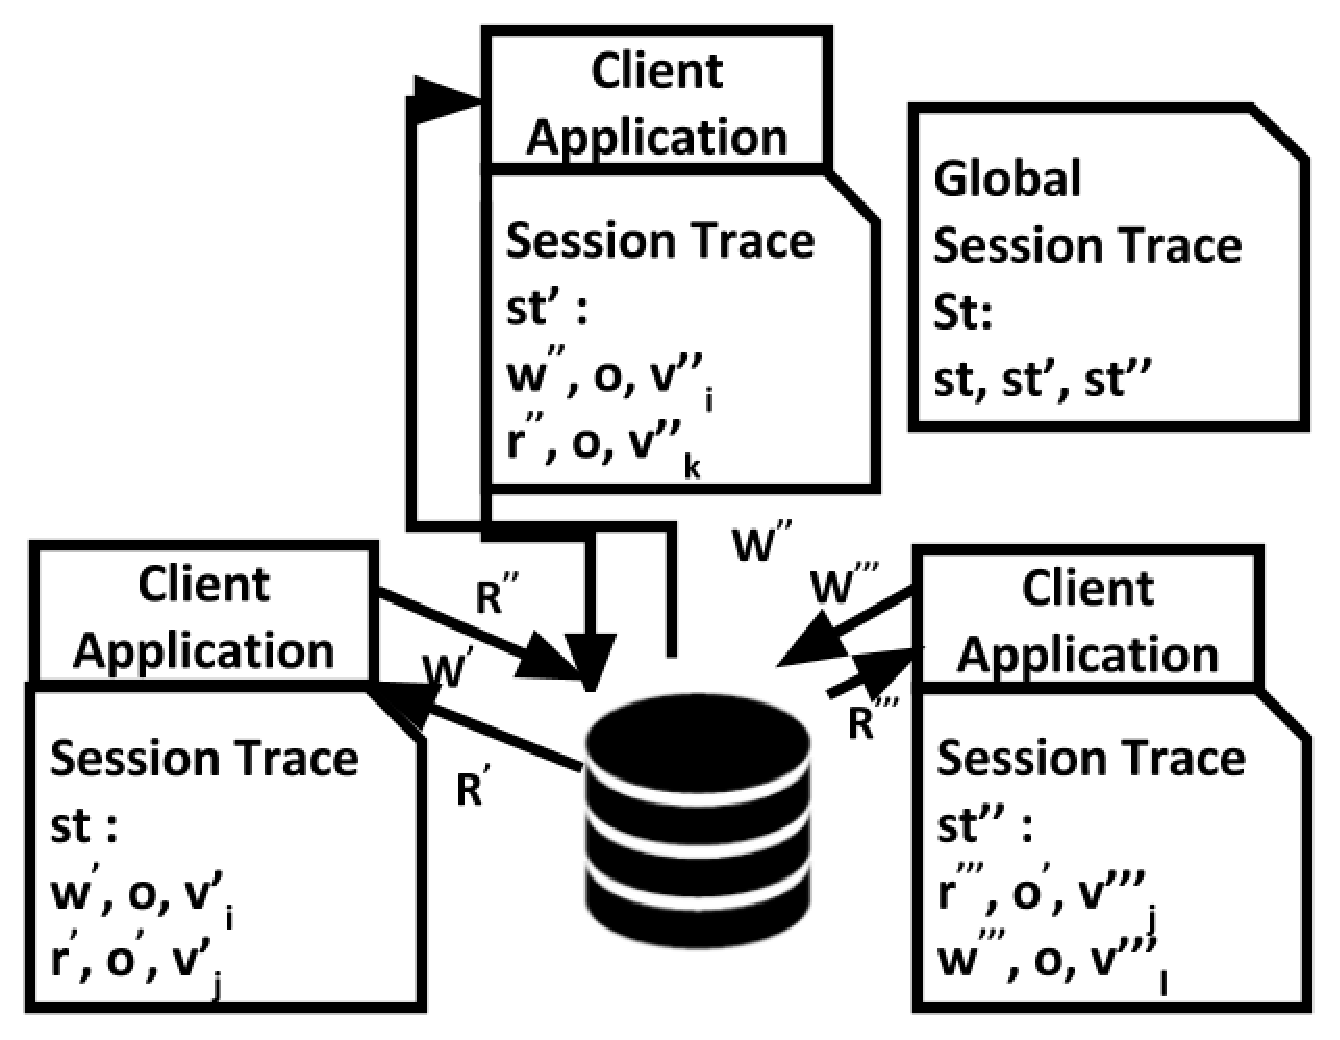
\includegraphics[height=3cm]{system.eps}
 
\end{frame}

\begin{frame}
\frametitle{Generalized form of ConSpec:}
	\begin{definition}{}\label{def:form0}
	Given a global session trace $\mathcal{S}_t$,
	% representing a global execution of all concurrent clients on a given storage
	%system,
	we say  that $\mathcal{S}_t$ satisfies a consistency model $\mathcal{C}$
	if there exists a partial order $\left( {\mathcal{O}_{St}}, \preccurlyeq \right)$ over the set ${\mathcal{O}_{St}}$ comprising operations  present in all session traces in $\mathcal{S}_t$, i.e.,  ${\mathcal{O}_{St}} = \bigcup_{st \in St} \{ o \mid o \in st \},$
	such that \\
	1) for every operation $\mathit{o}$ in  ${\mathcal{O}_{St}}$, %$\mathcal{S}_t$,
	its output is equal to the one obtained by executing the sequential specification of an  equivalent re-arrangement (i.e., permutation) %a linear extension of
	of the operations preceding $\mathit{o}$ in $\preccurlyeq$, \\
	% the same irrespective of the
	%%among operations preceding it in $\preccurlyeq$, %$\exists {\mathit{Op}^i}^{'}, {\mathit{Op}^j}^{'} \in \mathcal{S}_t:
	%{\mathit{Op}^i}^{'} \preccurlyeq {\mathit{Op}^j}^{'}\; \Rightarrow \;{\mathit{Op}^i}^{'} R {\mathit{Op}^j}^{'}$, %\; \vee \; v_i \sim v_j$,{\mathcal{O}_{St}}, \preccurlyeq
	and 2) $\left( {\mathcal{O}_{St}}, \preccurlyeq \right)$ obeys $E^S_C$, which is an LTL expression restricting $\left( {\mathcal{O}_{St}}, \preccurlyeq \right)$.
\end{definition}
\end{frame}

\begin{frame}
\frametitle{ConSpec Definition of the Consistency Model RYW}
	\begin{align}\label{eqn:RYW}
\begin{split}
%  \mathcal{E}^{s} = \forall  \mathit{st} \in \mathcal{S}_t, {W^i}^{'}, {R^j}^{'} \in \mathit{st}
%  \big( \left( {W^i}^{'} F {R^j}^{'} \in \mathit{st} \right)
% \Rightarrow \; \exists S_p \\
% \left(  {W^i}^{'} F {R^j}^{'} \in S_p \right)\big).
% \mathcal{E}^{s} = \forall  {W^i}^{'}, {R^j}^{'} \in \mathit{st}
%  \big( \left( {W^i}^{'} F {R^j}^{'} \in \mathit{st} \right)
% \Rightarrow \\
% \left(  {W^i}^{'} \preccurlyeq_{\mathit{st}+w} {R^j}^{'} \right)\big),
%E^S_C = \quad \forall st \in \mathcal{S}_t, \;  {W}'(x), {R}'(x) \in \mathit{st} : \\
E^S_C =  \forall x \in \mathcal{X}, \mathit{st} \in  \mathcal{S}_t, W_\mathit{st}^x, R_\mathit{st}^x \in \mathit{st}:
\\ \left( \square \left( W_\mathit{st}^x \rightarrow \lozenge R_\mathit{st}^x \right)
\rightarrow  W_\mathit{st}^x  \preccurlyeq_{\mathit{st}+w} R_\mathit{st}^x \right),
%C = \left( \not\exists {R^k}^{'}, {W^l}^{'} \in \mathcal{S}_t \right)   \big( %\left( {W^i}^{'} F {R^j}^{'} \in \mathit{st} \right) \wedge
%\left( {R^k}^{'} F {R^j}^{'} \in \mathit{st} \right)   \\ \wedge
%%\left(  \mathit{st}^{'} \in \mathcal{S}_t \right) \wedge
%\left( {W^l}^{'} F {W^i}^{'} \in \mathcal{S}_t \right)  %\big) \\
%\wedge \left(  {v^k}^{'} = {v^i}^{'} \right) \wedge  \big( \left( {v^j}^{'} = {v^l}^{'} \right) \vee \\
%\big( \left( {W^l}^{'} F {R^j}^{'} \in \mathcal{S}_t \right)  \wedge
%  \not\exists {W^m}^{'} \left( {W^l}^{'} F {W^m}^{'} F {R^j}^{'} \in \mathcal{S}_t \right) \big) \big).
\end{split}
\end{align}\\

Violation example:
$\mathit{st}_1$: $w(x,1), w'(x,2), r(x){2}, r'(x){1}$\\

Satisfaction example:
$\preccurlyeq_{\mathit{st}+w}^1$ = $W^x_{\mathit{st}} \preccurlyeq_{\mathit{st}+w}^1 W'^x_{\mathit{st}} \preccurlyeq_{\mathit{st}+w}^1 R^x_{\mathit{st}}
\preccurlyeq_{\mathit{st}+w}^1 R'^x_{\mathit{st}}$
\end{frame}

\begin{frame}
\frametitle{ConSpec Definition of the Sequential Consistency}
\begin{align}\label{eqn:SC}
\begin{split}
E^S_C =  %(\forall \mathit{st} \in \mathcal{S}_t, \; {\mathit{Op}}, {\mathit{Op}}'(x) \in \mathit{st}: \\
% \square\; \mathit{Op}(x) \operatorname{\it F}_\mathit{st} {\mathit{Op}}'(x) \Rightarrow  {\mathit{Op}}(x) \preccurlyeq {\mathit{Op}}'(x)) \quad
\forall x,y \in \mathcal{X}, \mathit{st} \in \mathcal{S}_t, O_\mathit{st}^x, O'^{y}_\mathit{st} \in \mathit{st}:  \\
\big( \square \left( O_\mathit{st}^x \rightarrow \lozenge O'^{y}_\mathit{st} \right)
%\forall \mathit{st} \in \mathcal{S}_t,\;  {R}'(x), {R}''(x) \in \mathit{st} : \\
%\square\; {R}'(x) \operatorname{\it F}_\mathit{st} {R}''(x)
\rightarrow O_\mathit{st}^x \preccurlyeq O'^{y}_\mathit{st}  \; \wedge
\\
\forall O'', O''' \in \mathcal{S}_t:
O'' \preccurlyeq O''' \vee O''' \preccurlyeq O'' \big). %\\
%\left({\mathit{Op}}'' \prec {\mathit{Op}}'''  \vee  {\mathit{Op}}'''  \preccurlyeq {\mathit{Op}}''\right)
\end{split}
\end{align}\\

Violation example:
	$\mathit{st}_1^{''}$:   $w(x, 1), w'(x,99), r(y){1}$, and

$\mathit{st}_2^{''}$:  $w(y, 1), w'(y,99), r(x){1}$\\

Satisfaction example:
$\mathit{st}_1^{''}$:   $w(x, 1), r(x){1}$, and

$\mathit{st}_2^{''}$:  $w(x, 2), r(x){2}, r(x){1}$
\end{frame}

\begin{frame}
\frametitle{Extending CAP Theorem}
\begin{theorem}[Generalized CAP theorem]\label{thrm:capan}
	In an asynchronous system, 
	 the following holds:
	$\forall \mathcal{S}_{it} \; \forall \preccurlyeq \in \Pi(\mathcal{S}_{it},E^S_C) \; \forall o \in max(\preccurlyeq) (\textsc{RemoveAllExceptSession}(\preccurlyeq,o) \in \Pi(\mathcal{S}_{it},E^S_C) ) $
	where we define {$\textsc RemoveAllExceptSession$} as a partial order where the maximum $o$ is only directly ordered after prior operations in the same session, i.e.:
	$\noindent {\textsc RemoveAllExceptSession}(\preccurlyeq,o(x)) \equiv \; \preccurlyeq \setminus \{ \langle o'(x),o(x) \rangle$ , where $\langle o'(x),o(x) \rangle$ belongs to the transitive reduction of $\preccurlyeq$, and $o'(x)$ does not belong to the same session as $o(x)\}$.
\end{theorem}
\end{frame}

\begin{frame}
\frametitle{ConSpec Checket Tool}
\begin{itemize}
	\item Spinroot based prototype Automated Verification Tools
 \item A global session trace is supplied to the tool as input
\item The Spin driver then runs the built-in model checker to check for counter-examples
\item Evaluated on two sets of traces: \\
1) generated by executing YCSB on top of a Cassandra cluster on Amazon aws,  \\
2)  obtained by executing the TPC-C benchmark on top of a MySQL database
\item Evaluation criteria: \\
A) How long the tool takes to check the consistency of a session trace, \\
B) how this validation time varies depending on the length (or size) of the trace, \\
C) How it compares to checking traces expressed in conventional syntaxes.
\end{itemize}
	
\end{frame}

\begin{frame}
\frametitle{Evaluation Results}

\begin{columns}
	
	\column{0.5\textwidth}
	\includegraphics[height=4cm]{conspecYCSBvarhist.eps}
	
	\column{0.5\textwidth}
	\includegraphics[height=4cm]{conspecTPCCvarhist.eps}
\end{columns}
Using the thread count parameter, we simulated a number of concurrent YCSB client threads executing the given workload,  where the number of clients corresponds to the value passed to this parameter.\\
Thus, each execution of the YCSB client with a given value of the thread parameter generates a global session trace consisting of multiple session traces, where each session trace comprises the entire sequence of operations performed from a specific client thread.

\end{frame}

\begin{frame}
\frametitle{Conclusions and Future Work}
\begin{itemize}
	\item A unified, simple specification that formalizes  consistency and models in an uniform syntax
	\item Equivalence to previous definitions
	\item Extension of CAP to different consistency models
	\item Explore combination of consistency and isolation
	\item Other advantages of LTL based definitions?
	\item Automated Verification Tool for verifying system Code against consistency and isolation specs
	\item Analyze the implications for system developers in terms of system design/development
\end{itemize}

\end{frame}
\end{document}
